\documentclass[11pt, oneside]{article} 
\usepackage{geometry}
\geometry{letterpaper} 
\usepackage{graphicx}
	
\usepackage{amssymb}
\usepackage{amsmath}
\usepackage{parskip}
\usepackage{color}
\usepackage{hyperref}

\graphicspath{{/Users/telliott_admin/Tex/png/}}
% \begin{center} 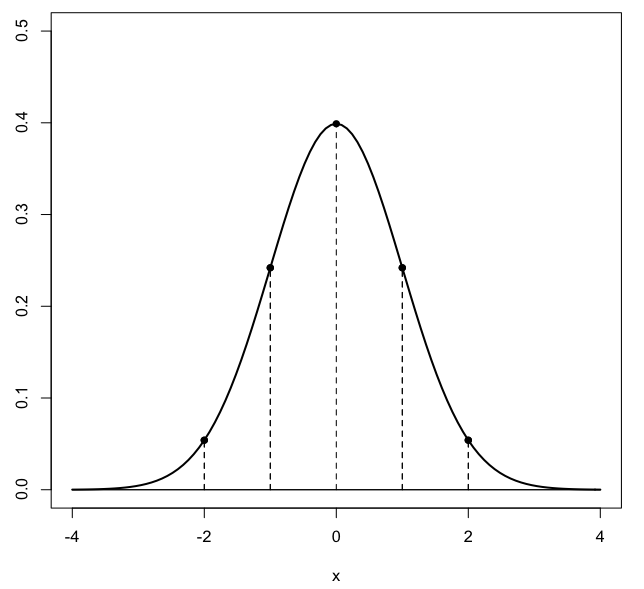
\includegraphics [scale=0.4] {gauss3.png} \end{center}

%break
\title{Euler's equation:  more}
\date{}

\begin{document}
\maketitle
\Large

\label{sec:Euler's_equation}

\subsection*{additional proofs}
Here are sketches of two different derivations of Euler's famous formula, both following Dunham's book about Euler.  He starts by simply admiring the formula
\[ e^{i\theta} = \cos \theta + i \sin \theta \]

If $\theta = \pi$, we have
\[ e^{i\pi} = -1 + 0 \]
\[ e^{i\pi}+ 1 = 0 \]
(what Feynman called "our jewel").

Dunham says in a video I saw that, if we were going to have a math party, we would invite these five numbers:  $0$ for arithmetic (additive identity), $1$ for multiplication (multiplicative identity), $\pi$ for geometry, $e$ for calculus, and $i$ for complex functions.

\subsection*{preliminary}
Using $x$ is a bit simpler notation, so that's what I'll do here
\[ e^{ix} = \cos x + i \sin x \]

Start with the definition of $i$
\[ i = \sqrt{-1} \]
Simple identities that come from it are:
\[ i^2 = - 1 \]
\[ -i^2 = 1 \]
\[ \frac{u}{i} = - i u \]

Having $i$ gives us new factorizations like
\[ a^2 + b^2 = (a + bi)(a - bi) \]
since the terms with $\pm \ abi$ cancel and $- i^2 = 1$.  
So
\[ 1 = \cos^2 x + \sin^2 x \]
\[ 1 = (\cos x + i \sin x) (\cos x - i \sin x) \]
Of course, we could switch sine and cosine here, but this is the convention.

\subsection*{derivation one}
Start with the inverse sine function:
\[ x = \sin^{-1} y \]
\[ y = \sin x \]
\[ dy = \cos x \ dx \]

Then we can make a trig substitution and say that the side adjacent to $x$ is $\sqrt{1-y^2}$ and so
\[ \cos x = \sqrt{1-y^2} \]

We're interested in the integral
\[ \int \frac{1}{\sqrt{1-y^2}} \ dy \]
which is just
\[ = \int \frac{1}{\cos x} \ \cos x \ dx = x \]

Now, Euler makes a complex change of variable
\[ y = iz \]
\[ \frac{1}{1-y^2} = \frac{1}{1+z^2} \]
So
\[ x = \int \frac{1}{\sqrt{1 - y^2}} \ dy = \int \frac{1}{\sqrt{1 + z^2}} \ i \ dz \]
we have converted the integral to having a plus sign under the square root and the answer is

\[ = i \ln \ (\sqrt{{1 + z^2}} + z) \]

This follows from a standard trig substitution but it's a bit complicated.  It can be checked by differentiating.  The derivative is $i$ times
\[ \frac{1}{\sqrt{1 + z^2} + z} \ (\frac{z}{ \sqrt{1+z^2}} + 1) \]
\[ = \frac{1}{\sqrt{1 + z^2} + z} \ (\frac{z + \sqrt{1+z^2}}{ \sqrt{1+z^2}}) \]
\[ = \frac{1}{\sqrt{1 + z^2}}  \]

Now, just undo the substitution:
\[ z = \frac{y}{i} = \frac{ \sin x}{i} \]
\[ \sqrt{1 + z^2} = \sqrt{1 - y^2} = \cos x \]
Hence our previous result
\[ x = i \ln \ (\sqrt{{1 + z^2}} + z) \]
is equivalent to
\[ x = i \ln \ (\cos x + \frac{\sin x}{i}) \]

Recall our two identities involving $i$.  The first one was
\[ \frac{u}{i} = - i u \]
So:
\[ x = i \ln \ (\cos x + \frac{\sin x}{i}) \]
\[ = i \ln \ (\cos x - i \sin x) \]
\[ ix = - \ln \ (\cos x - i \sin x) \]
\[ = \ln \ \frac{1}{(\cos x - i \sin x)} \]

Using the factorization given at the top
\[ \frac{1}{\cos u - i \sin u} = \cos u + i \sin u \]
We have that
\[ ix = \ln \ \frac{1}{(\cos x - i \sin x)}  = \ln \ (\cos x + i \sin x) \]
Exponentiate:
\[ e^{ix} = \cos x + i \sin x \]

\subsection*{derivation two}
Suppose we try this multiplication:
\[ (\cos s + i \sin s) (\cos t + i \sin t) \]
\[ = \cos s \cos t + i \sin s \cos t + i \cos s \sin t - \sin s \sin t \]
\[ = (\cos s \cos t - \sin s \sin t) + i (\sin s \cos t + \cos s \sin t) \]
\[ = \cos (s+t) + i \sin(s + t) \]

set $s=t$ and recall what we started with
\[ (\cos s + i \sin s)^2 = \cos 2s + i \sin 2s \]

In fact, Euler showed that this is true for fractional $n$ but I'll assume that part.
\[ (\cos s + i \sin s)^n = \cos ns  + i \sin ns \]

Now multiply the difference rather than the sum:
\[ (\cos s - i \sin s) (\cos t - i \sin t) \]
\[ = (\cos s \cos t - \sin s \sin t ) - i (\sin s \cos t + \sin t \cos s) \]
\[ = \cos(s+t) - i (\sin (s + t)) \]

again, with $s=t$
\[ ( \cos s - i \sin s)^2 = \cos 2s - i \sin 2s \]
\[ ( \cos s - i \sin s)^n = \cos ns - i \sin ns \]

Restate the two results:
\[ (\cos s + i \sin s)^n = \cos ns  + i \sin ns \]
\[ ( \cos s - i \sin s)^n = \cos ns - i \sin ns \]
Add them
\[ 2 \cos ns = (\cos s + i \sin s)^n + ( \cos s - i \sin s)^n \]

\subsection*{where the magic happens}
Let 
\[ s = \frac{x}{n} \]
As $n \rightarrow \infty$, $s \rightarrow 0$, and 
\[ \sin s \rightarrow s \] 
(by the famous limit from trigonometry)
\[ \cos s \rightarrow 1\]
\[ \cos x  = \cos ns \]

We had
\[ 2 \cos ns = (\cos s + i \sin s)^n + ( \cos s - i \sin s)^n \]
which becomes
\[ 2 \cos x =  (1 + i s)^n + (1 - i s)^n \  \]
\[ = (1 + \frac{ix}{n})^n + (1 - \frac{ix}{n})^n  \]

but from the standard limit developed in looking at the exponential
\[ e^{ix} = \lim_{n \rightarrow \infty} (1 + \frac{ix}{n})^n \]
hence
\[  2 \cos x  = e^{ix} + e^{-ix}  \]

We can just integrate this to obtain
\[  2i \sin x  = e^{ix} - e^{-ix} \]

Or by very similar manipulation to what's in the first part we can also obtain an expression for the sine:

\[ 2i \sin(ns) = (\cos s + i \sin s)^n - (\cos s - i \sin s)^n  \]
which will lead to the same thing
\[ 2i \sin x =  (e^{ix} - e^{-ix}) \]

Adding together
\[ 2(\cos x + i \sin x) = e^{ix} + e^{-ix} + e^{ix} - e^{-ix} \]
\[ \cos x + i \sin x = e^{ix} \]

\subsection*{check}
Before we stop, we can check the formula.  One way is to notice the connection between infinite series expansions for $e^x$:

\[ e^x = \sum_{n=0}^{\infty} \frac{x^n}{n!}  =  1 + x + \frac{x^2}{2!} + \frac{x^3}{3!} + \frac{x^4}{4!} \dots \]

sine:
\[ \sin x = x - \frac{x^3}{3!} + \frac{x^5}{5!} - \frac{x^7}{7!} \dots \]

and cosine:
\[ \cos x = 1 - \frac{x^2}{2!} + \frac{x^4}{4!} - \frac{x^6}{6!} \dots \]

These can almost be added together to give what we seek, except for the problem of the alternating signs.  What happens with $e^{ix}$?

\[ e^{ix} =  1 + ix + \frac{i^2x^2}{2!} + \frac{i^3x^3}{3!} + \frac{i^4x^4}{4!} \dots \]
\[ = 1 + ix - \frac{x^2}{2!} - i  \frac{x^3}{3!} + \frac{x^4}{4!} \dots \]

The pattern is 
\[  \sum_{n=0}^{\infty} i^n = 1 + i - 1 - i + 1 \dots \]

And we're there.  We just have to recognize that the pattern with $e^{ix}$ has $i \sin x$ so as we said
\[ e^{ix} = \cos x + i \sin x \]

\end{document}